\section{Метод моментов}

    Первым из методов, которые мы рассмотрим, будет метод моментов. Он основан на приравнивании теоретических характеристик распределения к выборочным. В случае пропусков, зависящих от данных, удобнее всего использовать следующие два равенства
    \begin{gather*}
        P\{obs_i = 1\} = \int_{-\infty}^{+\infty}p_\xi(x,\theta)(1 - m(x))\dd x = \frac{k}{n}, \\
        E\{x_i\} = \frac{\int_{-\infty}^{+\infty}xp_\xi(x,\theta)(1-m(x))\dd x}{\int_{-\infty}^{+\infty}p_\xi(x,\theta)(1-m(x))\dd x} = \frac{\sum_{obs_i = 1}x_i}{k},
    \end{gather*}
    где $k$ --- количество наблюдаемых значений в выборке.

    Сначала посмотрим, как изменится вид уравнений в различных случаях с пропусками.

    \paragraph{1. Случайные пропуски.} В этом случае $m(x) \equiv c,\ 0 < c < 1$ и уравнения 
    примут следующий вид
    \begin{gather*}
        \frac{k}{n} = \int_{-\infty}^{+\infty}p_\xi(x,\theta)(1-m(x))\dd x = 
            (1-c)\int_{-\infty}^{+\infty}p_\xi(x,\theta)\dd x = 1-c \\
        \frac{\sum_{obs_i = 1}x_i}{n} = 
            \frac{\int_{-\infty}^{+\infty}xp_\xi(x,\theta)(1-m(x))\dd x}%
                {\int_{-\infty}^{+\infty}p_\xi(x,\theta)(1-m(x))\dd x} = E\{\xi\}
    \end{gather*}
    Из первого уравнения пропала $\theta$, поэтому его нельзя использовать. Вместо него можно
    составить уравнение для момента порядка 2 или выше. Второе же уравнение в итоге ничем не отличается от
    соответствующего уравнения в случае без пропусков.

    \paragraph{2. Цензурирование.} Рассматриваем функцию вероятности пропуска
    \begin{equation*}
        m(x) = \begin{cases}
            0, & x < c \\
            1, & x \ge c
        \end{cases}.
    \end{equation*}
    В таком случае уравнения примут вид
    \begin{gather*}
        \int_{-\infty}^{c}p_\xi(x,\theta)\dd x = \frac{k}{n}, \\
        \frac{\int_{-\infty}^{c}xp_\xi(x,\theta)\dd x}{\int_{-\infty}^{c}p_\xi(x,\theta)\dd x} = \frac{\sum_{obs_i = 1}x_i}{n}
    \end{gather*}

    \paragraph{3. Кусочно-постоянная функция пропусков.} К примеру, возьмем функцию
    \begin{equation*}
        m(x) = \begin{cases}
            0, & x < a \\
            \frac12, & a \le x < b \\
            1, & x \ge b
        \end{cases}.
    \end{equation*}
    Подставив в уравнения баланса, получим
    \begin{gather*}
        \int_{-\infty}^{a}p_\xi(x,\theta)\dd x + \frac12\int_{a}^{b}p_\xi(x,\theta)\dd x = \frac{k}{n} \\
        \frac{\int_{-\infty}^{a}xp_\xi(x,\theta)\dd x + \frac12\int_{a}^{b}xp_\xi(x,\theta)\dd x}%
            {\int_{-\infty}^{c}p_\xi(x,\theta)\dd x + \frac12\int_{a}^{b}p_\xi(x,\theta)\dd x} = \frac{\sum_{obs_i = 1}x_i}{n}
    \end{gather*}
    Для решения сначала применим метод к распределению с одним параметром, например к экспоненциальному
    \begin{equation*}
        p(x,\theta) = \begin{cases}
                \theta e^{-\theta x}, &  x \ge 0 \\
                0,                    &  x < 0 
            \end{cases}, \quad \theta > 0.
    \end{equation*}
    В случаях 2 и 3 уравнения усложняются, в особенности тем, что во втором уравнении слева имеем частное
    двух интегралов, зависящих от $\theta$. 

    Теперь проверим метод моментов на практике. Возьмем параметр $\theta = 1$ и функцию модели пропусков
    \begin{equation*}
        m(x) = \begin{cases}
                1,       & x < 1 \\
                \frac12, & 1 \le x \le 2 \\
                0,       & x > 2
            \end{cases}
    \end{equation*}
    и проведем компьютерный эксперимент, аналогичный тому, который проводился для метода <<игнорирования пропусков>>. 
    Замечу, что здесь достаточно только одного из двух уравнений метода моментов. В таком случае можно решать его методом дихотомии, предполагая, что функция зависимости интеграла $\int_{-\infty}^{+\infty}p_\xi(x,\theta)m(x)\dd x$ от параметра $\theta$ монотонна.

    На рисунках 3 и 4 показаны оценки и их вариация для разных объемов выборки.
    \begin{figure}[H]
        \subcaptionbox*{Рисунок 3}[.49\linewidth]{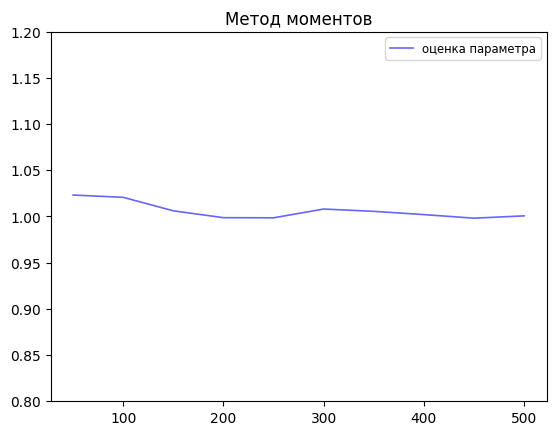
\includegraphics[width=\linewidth]{pict3.png}}
        \hfill
        \subcaptionbox*{Рисунок 4}[.49\linewidth]{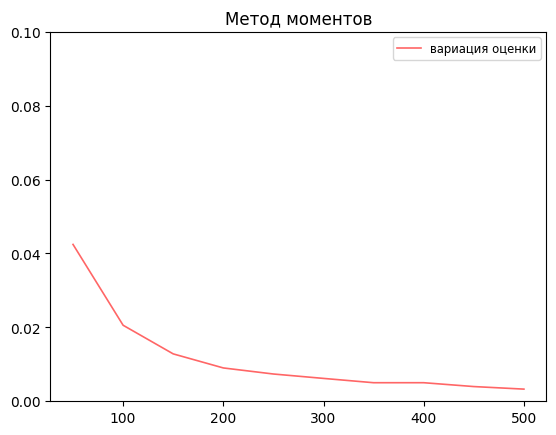
\includegraphics[width=\linewidth]{pict4.png}}
    \end{figure}
    Как видим, метод достаточно точен и даже при небольшом объеме выборки средняя вариация не превысила значения 0.05.

    Теперь попробуем таким же образом применить этот метод к нормальному распределению c параметрами $a = 0.7$ и $\sigma = 0.8$. 
    Так как параметра два, придется решать систему из двух уравнений, приведенных в начале главы. Это гораздо сложнее, чем в случае с одним параметром, поэтому для нахождения решения использовались инструменты языка Python (в котором реализован метод сопряженных направлений).

    На рисунках 5 и 6 показаны оценка и вариация соответственно для параметров распределения. Видим, что для нормального распределения метод тоже работает.
    \begin{figure}[H]
        \subcaptionbox*{Рисунок 5}[.49\linewidth]{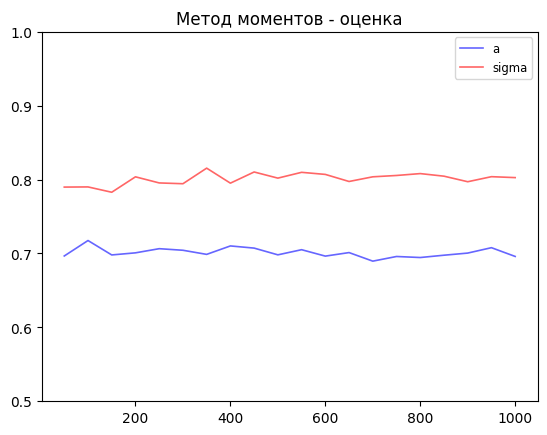
\includegraphics[width=\linewidth]{pict5.png}}
        \hfill
        \subcaptionbox*{Рисунок 6}[.49\linewidth]{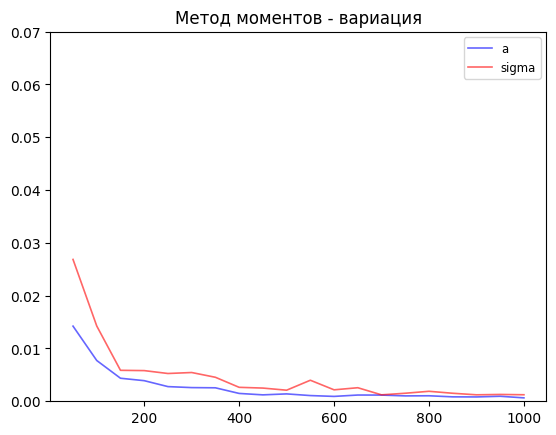
\includegraphics[width=\linewidth]{pict6.png}}
    \end{figure}